% ----------------------------------------------------------------------------------------------------- %
% Lista 1 de PDS - Baseado na classe UFTeX
% ----------------------------------------------------------------------------------------------------- %

\documentclass[tcc]{classe_uftex/uftex}
% ---- Esse comando cria o nome uftex estilizado
\newcommand\uftex{UF\TeX}

\usepackage{lipsum}
\usepackage{tikz}
\usepackage[siunitx]{circuitikz}
\usetikzlibrary{arrows}

\usepackage[alf,abnt-emphasize=bf]{referencias_abnt/abntex2cite}
\usepackage{xcolor}
\usepackage{mathptmx} % Times New Roman (ABNT)
\usepackage{float}
\usepackage{amsmath, amssymb}

\renewcommand{\lstlistingname}{Código}
\renewcommand{\lstlistlistingname}{Lista de Códigos}

\definecolor{codegreen}{rgb}{0,0.6,0}
\definecolor{codegray}{rgb}{0.5,0.5,0.5}
\definecolor{codepurple}{rgb}{0.58,0,0.82}
\definecolor{backcolour}{rgb}{0.98,0.98,0.98}
\definecolor{codeblue}{rgb}{0,0,0.8}

\lstset{
  language=Matlab,
  backgroundcolor=\color{backcolour},   
  commentstyle=\color{codegreen},
  keywordstyle=\color{codeblue}\bfseries,
  numberstyle=\normalsize\color{codegray},
  stringstyle=\color{codepurple},
  basicstyle=\ttfamily\small\color{black},
  breakatwhitespace=false,         
  breaklines=true,                 
  captionpos=b,                    
  keepspaces=true,                 
  numbers=left,                    
  numbersep=12pt,                  
  showspaces=false,                
  showstringspaces=false,
  showtabs=false,                  
  tabsize=2,
  frame=lines,
  rulecolor=\color{black!30},
  xleftmargin=20pt,
  framexleftmargin=5pt,
  aboveskip=20pt,
  belowskip=20pt
}

\renewcommand{\backrefpagesname}{}
\renewcommand{\backref}{}
\renewcommand*{\backrefalt}[4]{}

% ---- Ajuste para transformar a capa de TCC em Relatório e numeração no rodapé
\makeatletter
\renewcommand*{\ps@plain}{%
  \let\@mkboth\@gobbletwo
  \let\@oddhead\@empty
  \def\@oddfoot{%
    \reset@font
    \hfil
    \thepage
  }%
  \let\@evenhead\@empty
  \let\@evenfoot\@oddfoot
}

\renewcommand\frontpage@maintext{
  \sloppy\nohyphens{Lista de Exercícios apresentada à disciplina de Processamento Digital de Sinais do curso de \local@deptname\ da \local@universityname .

 \vspace{.5cm}
  \nohyphens{%
    \count1=0
    \@whilenum \count1<\@advisor \do{%
    \ifcase\count1 % same as \ifnum0=\count1
        Professor: \csname uftAdvisorDegree:\the\count1 \endcsname \ 
        \csname uftAdvisorName:\the\count1 \endcsname \ 
        \csname uftAdvisorSurname:\the\count1 \endcsname \ \par
    \else
        \local@coadvisorstring: \csname uftAdvisorDegree:\the\count1 \endcsname \ 
        \csname uftAdvisorName:\the\count1 \endcsname \ 
        \csname uftAdvisorSurname:\the\count1 \endcsname \ \par
    \fi
    \advance\count1 by 1}
  } \par
}
}
\makeatother

% ---- Início do documento
\begin{document}
  % ---- Descrição do título do trabalho 
  \title{Lista de Exercícios 1: Sinais e Sistemas Discretos}
  % ---- Nome do autor ou autores do trabalho
  \author{Maurício}{Moura de Carvalho}
  % ---- Nome do orientador do trabalho.
  \advisor{Prof.}{Ivan}{Ney Alvizuri Romani}{Dr.}

  % ---- Departamento
  \department{EE} % ou o departamento correto
  
  % ---- Data
  \date{30}{03}{2026}
  
  % ---- Palavras-chaves
  \keyword{Processamento Digital de Sinais}
  \keyword{Exercícios}
  \keyword{Sistemas Discretos}

  % ---- Palavras-chaves em inglês
  \foreignkeyword{Digital Signal Processing}
  \foreignkeyword{Exercises}
  \foreignkeyword{Discrete Systems}
  
  \maketitle
  \frontmatter

  % ---- Cria o sumário
  \tableofcontents 
  
  % --- Marca o inicio dos elementos textuais
  \mainmatter
  \setcounter{page}{1} 
  \onehalfspacing

% ----------------------------------------------------------------------------------------------------- %
% Exercícios
% ----------------------------------------------------------------------------------------------------- %

\chapter{Exercícios Solucionados}

\section{Questão 1: Periodicidade de Sinais}

\textbf{Enunciado:} Determine se os seguintes sinais são periódicos ou não. Se forem periódicos, encontre o período fundamental $N$.

\begin{enumerate}
    \item[\textbf{a)}] $x[n] = (-1)^n$
    \item[\textbf{b)}] $x[n] = \text{sen}(40\pi n/105)$
    \item[\textbf{c)}] $x[n] = \cos(2n)$
    \item[\textbf{d)}] $x[n] = \cos(2\pi n)$
    \item[\textbf{e)}] $x[n] = \cos(\frac{7}{15}\pi n)$
    \item[\textbf{f)}] $x[n] = \cos(\frac{1}{5}\pi n)\text{sen}(\frac{1}{3}\pi n)$
    \item[\textbf{g)}] $x[n] = \sum_{k=-\infty}^{\infty} \{\delta[n-3k] + \delta[n-k^2]\}$
    \item[\textbf{h)}] $x[n]$ descrito na Figura 1.
\end{enumerate}

\subsection*{Solução}

Para um sinal discreto ser periódico, a relação $\frac{\Omega_0}{2\pi}$ deve ser um número racional $\frac{m}{N}$, onde $m, N \in \mathbb{Z}$. O período fundamental é o menor $N$.

\begin{itemize}
    \item[\textbf{a)}] $x[n] = (-1)^n = \cos(\pi n)$. Aqui $\Omega_0 = \pi$.
    $\frac{\pi}{2\pi} = \frac{1}{2}$. É racional ($m=1, N=2$). 
    \textbf{Periódico, $N = 2$}.

    \item[\textbf{b)}] $x[n] = \text{sen}\left(\frac{40\pi n}{105}\right) = \text{sen}\left(\frac{8\pi n}{21}\right)$. Aqui $\Omega_0 = \frac{8\pi}{21}$.
    $\frac{8\pi/21}{2\pi} = \frac{4}{21}$. É racional ($m=4, N=21$).
    \textbf{Periódico, $N = 21$}.

    \item[\textbf{c)}] $x[n] = \cos(2n)$. Aqui $\Omega_0 = 2$.
    $\frac{2}{2\pi} = \frac{1}{\pi}$. Como $\pi$ é irracional, a relação não é racional.
    \textbf{Não periódico}.

    \item[\textbf{d)}] $x[n] = \cos(2\pi n)$. Como $n \in \mathbb{Z}$, $x[n] = 1$ para todo $n$.
    $\frac{2\pi}{2\pi} = 1$. É racional ($m=1, N=1$).
    \textbf{Periódico, $N = 1$}.

    \item[\textbf{e)}] $x[n] = \cos\left(\frac{7\pi n}{15}\right)$. Aqui $\Omega_0 = \frac{7\pi}{15}$.
    $\frac{7\pi/15}{2\pi} = \frac{7}{30}$. É racional ($m=7, N=30$).
    \textbf{Periódico, $N = 30$}.

    \item[\textbf{f)}] $x[n] = \cos\left(\frac{\pi n}{5}\right)\text{sen}\left(\frac{\pi n}{3}\right)$. Usando a identidade trigonométrica de produto-para-soma:
    $x[n] = \frac{1}{2}\left[\text{sen}\left(\frac{8\pi n}{15}\right) + \text{sen}\left(\frac{2\pi n}{15}\right)\right]$.
    Para $\Omega_1 = \frac{8\pi}{15}$, $N_1 = \frac{30}{8} \cdot m \Rightarrow N_1 = 15$ ($m=4$).
    Para $\Omega_2 = \frac{2\pi}{15}$, $N_2 = \frac{30}{2} \cdot m \Rightarrow N_2 = 15$ ($m=1$).
    O período é $\text{mmc}(N_1, N_2) = 15$.
    \textbf{Periódico, $N = 15$}.

    \item[\textbf{g)}] $x[n] = \sum_{k=-\infty}^{\infty} \delta[n-3k] + \sum_{k=-\infty}^{\infty} \delta[n-k^2]$.
    A primeira soma é o trem de impulsos periódico com $N=3$. No entanto, a segunda soma possui impulsos nos instantes $n = k^2$ ($0, 1, 4, 9, 16 \dots$). Como a distância entre os impulsos aumenta ($1, 3, 5, 7 \dots$), a sequência não se repete.
    \textbf{Não periódico}.

    \item[\textbf{h)}] Analisando a Figura 1, observa-se um padrão que se repete a cada 10 amostras. Existe um grupo de 3 impulsos centrados em múltiplos de $10$ ($n=0, 10, 20 \dots$) e um grupo de 2 impulsos centrados nos deslocamentos de $5$ ($n=5, 15, 25 \dots$).
    \textbf{Periódico, $N = 10$}.
\end{itemize}

\begin{figure}[H]
\centering
\begin{tikzpicture}[scale=0.45]
    % Eixos
    \draw[->] (-12.5, 0) -- (23.5, 0) node[right] {$n$};
    \draw[->] (0, -0.5) -- (0, 2) node[above] {$x[n]$};
    
    % Ticks e referencias
    \foreach \x in {-10, -5, 0, 5, 10, 15, 20}
        \draw (\x, 0.1) -- (\x, -0.1) node[below=4pt] {\small $\x$};
        
    \draw (0.1, 1) -- (-0.1, 1) node[left] {\small 1};
    
    % Zeros (amostras com valor 0)
    \foreach \x in {-12, -8, -7, -4, -3, -2, 2, 3, 6, 7, 8, 12, 13, 16, 17, 18, 22} {
        \draw[blue, fill=white] (\x, 0) circle (2pt);
    }
    
    % Uns (amostras com valor 1)
    \foreach \x in {-11, -10, -9, -6, -5, -1, 0, 1, 4, 5, 9, 10, 11, 14, 15, 19, 20, 21} {
        \draw[blue] (\x, 0) -- (\x, 1);
        \draw[blue, fill=white] (\x, 1) circle (2pt);
    }
    
    \node[blue] at (-13.5, 0) {\dots};
    \node[blue] at (24.5, 0) {\dots};
\end{tikzpicture}
\caption{Sinal descrito no item h).}\label{fig:f1}
\end{figure}

\section{Questão 2: Operações Básicas de Sinais}

\textbf{Enunciado:} Considere os sinais discretos $x[n]$ e $y[n]$ apresentadas nas Figuras 2 e 3 respectivamente.

\begin{figure}[H]
\centering
\begin{minipage}{0.48\textwidth}
\centering
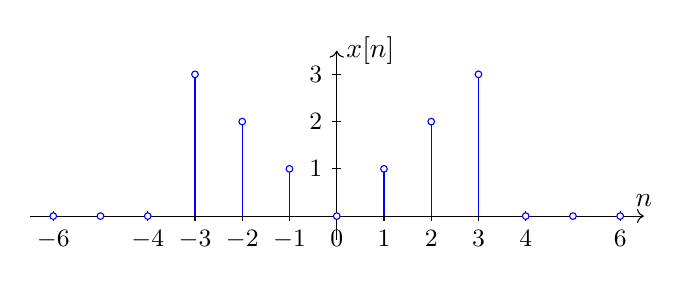
\begin{tikzpicture}[scale=0.6]
    % Eixos
    \draw[->] (-6.5, 0) -- (6.5, 0) node[above] {$n$};
    \draw[->] (0, -0.5) -- (0, 3.5) node[right] {$x[n]$};
    
    % Ticks
    \foreach \x in {-6, -4, -3, -2, -1, 0, 1, 2, 3, 4, 6}
        \draw (\x, 0.1) -- (\x, -0.1) node[below] {\small $\x$};
    \foreach \y in {1, 2, 3}
        \draw (0.1, \y) -- (-0.1, \y) node[left] {\small $\y$};
        
    % Hastes e pontos x[n]
    \foreach \x/\y in {-6/0, -5/0, -4/0, -3/3, -2/2, -1/1, 0/0, 1/1, 2/2, 3/3, 4/0, 5/0, 6/0} {
        \draw[blue] (\x, 0) -- (\x, \y);
        \draw[blue, fill=white] (\x, \y) circle (2pt);
    }
\end{tikzpicture}
\caption{Sinal $x[n]$.}\label{fig:f2}
\end{minipage}
\hfill
\begin{minipage}{0.48\textwidth}
\centering
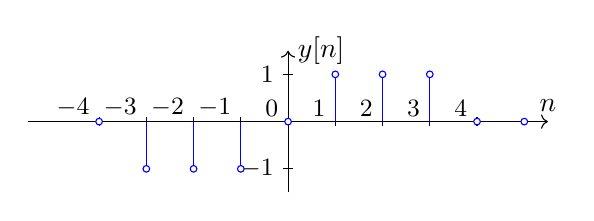
\begin{tikzpicture}[scale=0.6]
    % Eixos
    \draw[->] (-5.5, 0) -- (5.5, 0) node[above] {$n$};
    \draw[->] (0, -1.5) -- (0, 1.5) node[right] {$y[n]$};
    
    % Ticks
    \foreach \x in {-4, -3, -2, -1, 0, 1, 2, 3, 4}
        \draw (\x, 0.1) -- (\x, -0.1) node[above left] {\small $\x$};
    \foreach \y in {-1, 1}
        \draw (0.1, \y) -- (-0.1, \y) node[left] {\small $\y$};
        
    % Hastes e pontos y[n]
    \foreach \x/\y in {-4/0, -3/-1, -2/-1, -1/-1, 0/0, 1/1, 2/1, 3/1, 4/0, 5/0} {
        \ifnum \y=0
            \draw[blue, fill=white] (\x, \y) circle (2pt);
        \else
            \draw[blue] (\x, 0) -- (\x, \y);
            \draw[blue, fill=white] (\x, \y) circle (2pt);
        \fi
    }
\end{tikzpicture}
\caption{Sinal $y[n]$.}\label{fig:f3}
\end{minipage}
\end{figure}

Calcule os seguintes sinais:
\begin{enumerate}
    \item[\textbf{a)}] $x[2n]$
    \item[\textbf{b)}] $x[3n-1]$
    \item[\textbf{c)}] $y[1-n]$
    \item[\textbf{d)}] $y[2-2n]$
    \item[\textbf{e)}] $x[n-2] + y[n+2]$
    \item[\textbf{f)}] $x[2n] + y[n-4]$
    \item[\textbf{g)}] $x[n+2]y[n-2]$
    \item[\textbf{h)}] $x[3-n]y[n]$
\end{enumerate}

\subsection*{Solução}

Para determinar as sequências resultantes, analisa-se a amplitude de $x[n]$ e $y[n]$ em cada instante temporal. Ambos os sinais foram apresentados zerados para valores de índice de tempo que não contenham hastes ativas. Observando os gráficos, obtemos:

$x[n] = 3\delta[n+3] + 2\delta[n+2] + \delta[n+1] + \delta[n-1] + 2\delta[n-2] + 3\delta[n-3]$

$y[n] = -\delta[n+3] - \delta[n+2] - \delta[n+1] + \delta[n-1] + \delta[n-2] + \delta[n-3]$

\begin{itemize}
    \item[\textbf{a)}] $x[2n]$ é uma decimação que descarta amostras ímpares.
    $x[0] = 0$; $x[-2] = 2$; $x[2] = 2$. Restante igual a 0.
    \textbf{Resultado:} $x[2n] = 2\delta[n+1] + 2\delta[n-1]$

    \item[\textbf{b)}] $x[3n-1]$. Apenas os índices $n$ inteiros que tornem $(3n-1) \in \{-3,-2,-1,1,2,3\}$ revelarão valores.
    Para $n=0 \Rightarrow 3(0)-1 = -1 \Rightarrow x[-1] = 1$.
    Para $n=1 \Rightarrow 3(1)-1 = 2 \Rightarrow x[2] = 2$.
    \textbf{Resultado:} $x[3n-1] = \delta[n] + 2\delta[n-1]$

    \item[\textbf{c)}] $y[1-n]$ envolve inversão no tempo ($n \to -n$) seguida de deslocamento para a direita de 1 unidade temporal. Valores que estavam em instante $k$ vão para $n = 1-k$.
    \textbf{Resultado:} $y[1-n] = \delta[n+2] + \delta[n+1] + \delta[n] - \delta[n-2] - \delta[n-3] - \delta[n-4]$

    \item[\textbf{d)}] $y[2-2n]$ é decimação e inversão simultaneamente. Apenas valores pares de deslocamentos fornecerão resultados não nulos para $y$.
    Para $n=0 \Rightarrow y[2] = 1$.
    Para $n=2 \Rightarrow y[-2] = -1$.
    \textbf{Resultado:} $y[2-2n] = \delta[n] - \delta[n-2]$

    \item[\textbf{e)}] $x[n-2] + y[n+2]$ soma, instante a instante, dos vetores atrasado e adiantado, respectivamente.
    $x$ atinge pico de amplitude 3 nos instantes $n = -1$ e $n = 5$.
    $y$ avança tornando seus valores negativos situados em $n \in \{-5, -4, -3\}$ e os positivos em $n \in \{-1, 0, 1\}$.
    Sobreposição ocorre apenas em $n=-1 \Rightarrow (-1 \cdot (-1) \text{ não, era sinal}) \dots$. Na verdade, para $n=-1$, temos $x[-3]=3$ somado a $y[1]=1 \Rightarrow 4$.
    \textbf{Resultado (apenas não nulos):} $\{-5 \to -1; \, -4 \to -1; \, -3 \to -1; \, -1 \to 4; \, 0 \to 3; \, 1 \to 2; \, 3 \to 1; \, 4 \to 2; \, 5 \to 3\}$

    \item[\textbf{f)}] $x[2n] + y[n-4]$ soma-se o resultado de $x[2n]$ isolado, o qual opera em $n \in \{-1, 1\}$, ao vetor isolado com seu atraso padrão de 4 no tempo.
    \textbf{Resultado:} $n=-1 \Rightarrow 2$, \quad $n=1 \Rightarrow 2 - 1 = 1$, \quad $n=2 \to -1$, \quad $n=3 \to -1$, \quad $n=5 \to 1$, \quad $n=6 \to 1$, \quad $n=7 \to 1$.

    \item[\textbf{g)}] $x[n+2]y[n-2]$ consiste na multiplicação direta no tempo das amplitudes nos índices coincidentes de ambos sinais deslocados opostamente.
    \textbf{Resultado:} Apenas instantes $\{-1, 0, 1\}$ estão intercalados entre eles com área não vazia, logo: $= -\delta[n+1] -2\delta[n] -3\delta[n-1]$

    \item[\textbf{h)}] $x[3-n]y[n]$ multiplicam-se as intersecções. Apenas sobreposições em $n=1$ ($x[2] \times y[1] = 2$) e $n=2$ ($x[1] \times y[2] = 1$).
    \textbf{Resultado:} $2\delta[n-1] + \delta[n-2]$
\end{itemize}

\section{Questão 3: Propriedades de Sistemas}

\textbf{Enunciado:} Os sistemas a seguir têm a entrada $x[n]$ e saída $y[n]$ respectivamente. Determine se cada um deles é sem memória, est\'avel, causal, linear e invariante no tempo.

\begin{enumerate}
    \item[\textbf{a)}] $y[n] = 2x[n]u[n]$
    \item[\textbf{b)}] $y[n] = \sum_{k=-\infty}^{n} x[k+2]$
    \item[\textbf{c)}] $y[n] = \cos(2\pi x[n+1]) + x[n]$
    \item[\textbf{d)}] $y[n] = x[n] \sum_{k=-\infty}^{\infty} \delta[n-2k]$
\end{enumerate}

\subsection*{Solução}

Para efetuar essa classificação, aplicamos as definições matemáticas formais das classificadores LTI em cada sistema submetido.

\begin{itemize}
    \item[\textbf{a)}] $y[n] = 2x[n]u[n]$
    \begin{itemize}
        \item \textit{Sem Memória:} Sim, pois $y[n]$ depende singularmente em cada instante simultâneo de amostragem no próprio $x[n]$, logo nunca olha para o tempo passado ou futuro.
        \item \textit{Estável:} Sim. $|y[n]| \le 2M < \infty$ caso $|x[n]| \le M$.
        \item \textit{Causal:} Sim (consequência natural de ser estático/sem memória).
        \item \textit{Linear:} Sim, respeita os postulados de superposição das amplitudes.
        \item \textit{Invariante no Tempo (LIT):} Não, pois o termo do tempo, imposto explicitamente pelo degrau multiplicativo $u[n]$, é de fato variante durante um deslocamento $x[n-k]$; não é possível fazer com que a máscara do degrau seja forçada a ser também deslocada por $k$ na relação global do atraso.
    \end{itemize}
    
    \item[\textbf{b)}] $y[n] = \sum_{k=-\infty}^{n} x[k+2]$
    \begin{itemize}
        \item \textit{Sem Memória:} Não, esse operador consiste num integrador infinito das amostras que compõe histórico (memória infinita); como a soma vai e passa em $x[n+2]$ se for rearmada temporalmente, precisa capturar instantes futuros independentemente.
        \item \textit{Estável:} Não. No caso de uma amostra constante ao longo do tempo (degrau de magnitude L), a somatória dispararia tendendo ao infinito.
        \item \textit{Causal:} Não. Pelo integrando $x[k+2]$, avaliando-se em $k=n$, a soma carece do valor adiantado em duas unidades no futuro ($x[n+2]$).
        \item \textit{Linear:} Sim.
        \item \textit{Invariante no Tempo (LIT):} Sim, as translações originadas nas entradas produzem ecos simétricos contínuos em equivalência e integrados nas saídas.
    \end{itemize}

    \item[\textbf{c)}] $y[n] = \cos(2\pi x[n+1]) + x[n]$
    \begin{itemize}
        \item \textit{Sem Memória:} Não. Pois existe demanda declarada por $x[n+1]$.
        \item \textit{Estável:} Sim, sempre contido graças as fronteiras extremas do cosseno $[-1, 1]$ somadas a amplitude da entrada avaliada.
        \item \textit{Causal:} Não, exige previsão algorítmica ou olhar à frente de uma amostra $n+1$.
        \item \textit{Linear:} Não, graças às disfunções puramente não elementais não é permitido decompor o argumento não-linear da raiz modular do cosseno por $ax_1 + bx_2$.
        \item \textit{Invariante:} Sim, atrasar a ordem globalmente altera harmoniosamente tudo para o bloco unificado como reflexo.
    \end{itemize}

    \item[\textbf{d)}] $y[n] = x[n] \sum_{k=-\infty}^{\infty} \delta[n-2k]$
    \begin{itemize}
        \item \textit{Sem Memória:} Sim, pois a sua computação foca num subconjunto da base com modulação $x[n]$ no instante e é apagado pelos zeros intercalados provenientes dos deltas.
        \item \textit{Estável:} Sim (nunca aumenta a massa pontual).
        \item \textit{Causal:} Sim.
        \item \textit{Linear:} Sim. Resultam de um produto da modulação que sustenta as leis aditivas diretas.
        \item \textit{Invariante no Tempo (LIT):} Não. Um simples eco não traduz perfeitamente. Um filtro indexando de dois em dois irá deixar passar um sinal deslocado dependendo dele cair numa posição par versus na ímpar restrito no deslocamento $n$.
    \end{itemize}
\end{itemize}

\section{Questão 4: Representação de Sistemas por Diagrama de Blocos}

\textbf{Enunciado:} A saída de um sistema de tempo discreto est\'a relacionada \`a sua entrada $x[n]$ da seguinte forma:
\begin{equation*}
    y[n] = a_0 x[n] + a_1 x[n-1] + a_2 x[n-2] + a_3 x[n-3]
\end{equation*}

Digamos que o operador $S^k$ denote um sistema que desloca a entrada $x[n]$ de $k$ unidades de tempo para produzir $x[n-k]$. Formule o operador $T$ para o sistema que relaciona $y[n]$ e $x[n]$. Logo, desenvolva uma representação em diagrama de blocos para $T$, usando (A) implementação em cascata e (B) implementação paralela. Finalmente mostre que esse sistema é BIBO est\'avel para todo $a_0$, $a_1$, $a_2$ e $a_3$.

\subsection*{Solução}

Isolando a definição do operador de retardo sistemático imposto como função formal em uma base matemática explícita, podemos descrever esse comportamento através de um modelo polinomial sobre a manipulação no atraso e mapeamentos esquemáticos.
A equação de diferenças da dinâmica proposta reflete a operação típica de um filtro digital FIR (Filtro de Resposta ao Impulso Finita).

O operador atraso base correspondente da equação resulta num fator de forma:
\begin{equation}
    T = a_0 + a_1 S + a_2 S^2 + a_3 S^3
\end{equation}

Uma rede em \textbf{Cascata} fatoriza o operador para agrupamentos seriados com base no conhecimento de fatores lineares de 1ª ordem, dispostos do tipo $T = (a_0) (1 - c_1 S)(1 - c_2 S)(...)$. Outrossim, para filtros FIR, pode-se tratar de um encadeamento direto (forma direta 1 delay-line) onde a saída dos atrasos são coletadas repetidas por sub-blocos somados em sequência. Diferente disso, para o diagrama da forma de \textbf{Configuração Paralela}, todos os atrasos base ocorrem espalhados no arranjo individual de forma independente na rede (somas de blocos). Como os $a_i$ são generalizados, um bloco de montagem explícita se fará presente nos ganhos unificados por nós de junção e acumuladores paralelos somando ao fim.

Para a validade da estabilidade BIBO em qualquer sistema do tipo de filtros de Resposta ao Impulso Finita (FIR), baseia-se na constatação analítica de que, caso aplicados coeficientes finitos em toda sua ordem da arquitetura (ou seja, $\forall |a_i| < \infty$), então a resposta impulsiva $h[n]$ total conterá apenas uma base de contagem limitada de amostras em série nulas no exterior:
\begin{equation}
    \sum_{n=-\infty}^\infty |h[n]| = |a_0| + |a_1| + |a_2| + |a_3| < \infty
\end{equation}
Portanto, as saídas nunca poderiam explodir irrestritamente sob restrições limitadas da excitação injetada $x[n]$. Logo, será essencialmente estritamente \textbf{Estável BIBO}.

\section{Questão 5: Operador Inverso}

\textbf{Enunciado:} O sinal de saída $y[n]$ de um sistema de tempo discreto est\'a relacionado ao seu sinal de entrada $x[n]$ da seguinte forma:
\begin{equation*}
    y[n] = x[n] + x[n-1] + x[n-2]
\end{equation*}

Admitamos que o operador $S$ denote um sistema que desloca sua entrada de uma unidade de tempo.
\begin{enumerate}
    \item[\textbf{a)}] Formule o operador $T$ para o sistema que relaciona $y[n]$ a $x[n]$.
    \item[\textbf{b)}] O operador $T^{-1}$ denota um sistema discreto que é o inverso do sistema. Como $T^{-1}$ é definido?
\end{enumerate}

\subsection*{Solução}

Substituindo sistematicamente a manipulação formal matemática de atraso analítico no elemento primário:

\begin{itemize}
    \item[\textbf{a)}] \textbf{Operador T}: Expressando os fatores deslocados pelo tempo como múltiplos operadores potentes de um mesmo polinômio de retardo elementar unitário padrão.
    \begin{equation}
        y[n] = x[n] + S\{x[n]\} + S^2\{x[n]\} \Rightarrow T = (1 + S + S^2)
    \end{equation}

    \item[\textbf{b)}] \textbf{Operador Inverso ($T^{-1}$)}: Representa formalmente qual o tipo de operador do cálculo equivalente com a pretensão em se restabelecer o sinal originário antes sob a excitação contínua para uma saída desejada anterior (ou seja, fazer $y[n] \to x[n]$). Matematicamente, isto produz o espelho da matriz de operação e assume:
    \begin{equation}
        T^{-1} = \frac{1}{1 + S + S^2}
    \end{equation}

    Na prática, o sistema direto era do tipo FIR (filtração por soma de média móvel não recursiva e de retardo temporizado elementar base). Já que $T^{-1}$ compreende frações algébricas polinomiais (em termos da variável de translação Z implícita), seu inverso denota-se imediatamente como um classificador \textbf{sistema dinâmico infinito recursivo (LIT IIR, Resposta ao Impulso Infinito)}. 
\end{itemize}

\section{Questão 6: Convolução e Resposta ao Impulso}

\textbf{Enunciado:} Um sistema discreto é tanto linear como invariante no tempo. Suponha que a saída devido à entrada $x[n]=\delta[n]$ seja dada pela Figura 4.

\begin{figure}[H]
\centering
\begin{minipage}{0.48\textwidth}
\centering
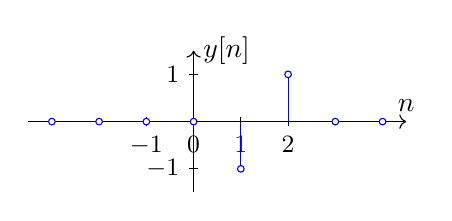
\begin{tikzpicture}[scale=0.6]
    % Eixos
    \draw[->] (-3.5, 0) -- (4.5, 0) node[above] {$n$};
    \draw[->] (0, -1.5) -- (0, 1.5) node[right] {$y[n]$};
    
    % Ticks
    \foreach \x in {-1, 0, 1, 2}
        \draw (\x, 0.1) -- (\x, -0.1) node[below] {\small $\x$};
    \foreach \y in {-1, 1}
        \draw (0.1, \y) -- (-0.1, \y) node[left] {\small $\y$};
        
    % Hastes e pontos y[n]
    \foreach \x/\y in {-3/0, -2/0, -1/0, 0/0, 1/-1, 2/1, 3/0, 4/0} {
        \ifnum \y=0
            \draw[blue, fill=white] (\x, \y) circle (2pt);
        \else
            \draw[blue] (\x, 0) -- (\x, \y);
            \draw[blue, fill=white] (\x, \y) circle (2pt);
        \fi
    }
\end{tikzpicture}
\caption{Figura 4: Resposta ao impulso.}\label{fig:f4}
\end{minipage}
\hfill
\begin{minipage}{0.48\textwidth}
\centering
\begin{tikzpicture}[scale=0.6]
    % Eixos
    \draw[->] (-3.5, 0) -- (4.5, 0) node[above] {$n$};
    \draw[->] (0, -1.5) -- (0, 2.5) node[right] {$x[n]$};
    
    % Ticks
    \foreach \x in {-2, -1, 0, 1, 2}
        \draw (\x, 0.1) -- (\x, -0.1) node[below left] {\small $\x$};
    \foreach \y in {-1, 1, 2}
        \draw (0.1, \y) -- (-0.1, \y) node[left] {\small $\y$};
        
    % Hastes e pontos x[n]
    \foreach \x/\y in {-3/0, -2/0, -1/1, 0/-1, 1/2, 2/0, 3/0, 4/0} {
        \ifnum \y=0
            \draw[blue, fill=white] (\x, \y) circle (2pt);
        \else
            \draw[blue] (\x, 0) -- (\x, \y);
            \draw[blue, fill=white] (\x, \y) circle (2pt);
        \fi
    }
\end{tikzpicture}
\caption{Figura 5: Sinal de entrada.}\label{fig:f5}
\end{minipage}
\end{figure}

\begin{enumerate}
    \item[\textbf{a)}] Encontre a saída devido a uma entrada $x[n]= \delta[n-1]$.
    \item[\textbf{b)}] Encontre a saída devido a uma entrada de $x[n]=2\delta[n]- \delta[n-2]$.
    \item[\textbf{c)}] Encontre a saída devido à entrada descrita na Figura 5.
\end{enumerate}

\subsection*{Solução}

Dado que o sistema é Linear e Invariante no Tempo (LIT), a saída para a entrada especial de teste $x[n] = \delta[n]$ por definição revela intrinsecamente a resposta ao impulso $h[n]$ do sistema completo. Interpretando a amplitude desenhada pelas hastes na Figura 4, a resposta ao impulso é mapeável pela soma linear dos termos não nulos:
\begin{equation}
    h[n] = -\delta[n-1] + \delta[n-2]
\end{equation}

Uma das propriedades fundamentais universais dos sistemas LIT é que a saída final $y[n]$ para qualquer formato arbitrário de entrada $x[n]$ é dada pelo operador linear da modelagem da soma de convolução: $y[n] = x[n] * h[n]$. Utilizaremos diretamente o superposicionamento ponderado e atrasado dessas repostas impulsórias limitadas para encontrar o sinal final requisitado.

\begin{itemize}
    \item[\textbf{a)}] Como o sinal foi deslocado puramente em 1 instante na fonte de entrada unitária $x[n] = \delta[n-1]$, a resposta por ser LIT apenas sofrerá igual retardo absoluto sem perdas ou distorções de módulo:
    \begin{equation}
        y[n] = h[n-1] = -\delta[n-2] + \delta[n-3]
    \end{equation}

    \item[\textbf{b)}] Para a entrada combinada $x[n] = 2\delta[n] - \delta[n-2]$, propagamos cada impulso isoladamente dentro das premissas de superposição de respostas como $y[n] = 2h[n] - h[n-2]$. Expansão por substituição direta no tempo das saídas primitivas em eco:
    \begin{align*}
        2h[n] &= 2(-\delta[n-1] + \delta[n-2]) = -2\delta[n-1] + 2\delta[n-2] \\
        -h[n-2] &= -(-\delta[n-3] + \delta[n-4]) = \delta[n-3] - \delta[n-4]
    \end{align*}
    Sintetizando ambas contribuições conjuntas:
    \begin{equation}
        y[n] = -2\delta[n-1] + 2\delta[n-2] + \delta[n-3] - \delta[n-4]
    \end{equation}

    \item[\textbf{c)}] Pela observação extraída do gráfico amostral explícito da Figura 5, percebe-se que seu o sinal de entrada equacionado é na verdade dado em componentes esparsos:
    \begin{equation}
        x[n] = \delta[n+1] - \delta[n] + 2\delta[n-1]
    \end{equation}
    A saída total equivalente será forçada baseando-se estritamente na homogeneidade, linearidade e invariância, sendo: $y[n] = h[n+1] - h[n] + 2h[n-1]$. Aplicando aditividade do operador nas componentes:
    \begin{align*}
        h[n+1] &= -\delta[n] + \delta[n-1] \\
        -h[n] &= \delta[n-1] - \delta[n-2] \\
        2h[n-1] &= -2\delta[n-2] + 2\delta[n-3]
    \end{align*}
    Condensando e agrupando os termos nas amostras de tempo sincrônicas (mesmos impulsos temporizados em evidência) ter-se-á:
    \begin{equation}
        y[n] = -\delta[n] + 2\delta[n-1] - 3\delta[n-2] + 2\delta[n-3]
    \end{equation}
\end{itemize}

\chapter{Conclusão}

As resoluções apresentadas permitem consolidar o conhecimento teórico-prático sobre o domínio discreto...

% ----------------------------------------------------------------------------------------------------- %
\backmatter 
\singlespacing   
% ----------------------------------------------------------------------------------------------------- %
\bibliography{lista_1}

\end{document}
